\documentclass[tikz,border=8pt]{standalone}
\usepackage{amsmath,amssymb}
\usetikzlibrary{arrows.meta,automata,positioning,quotes}
\begin{document}
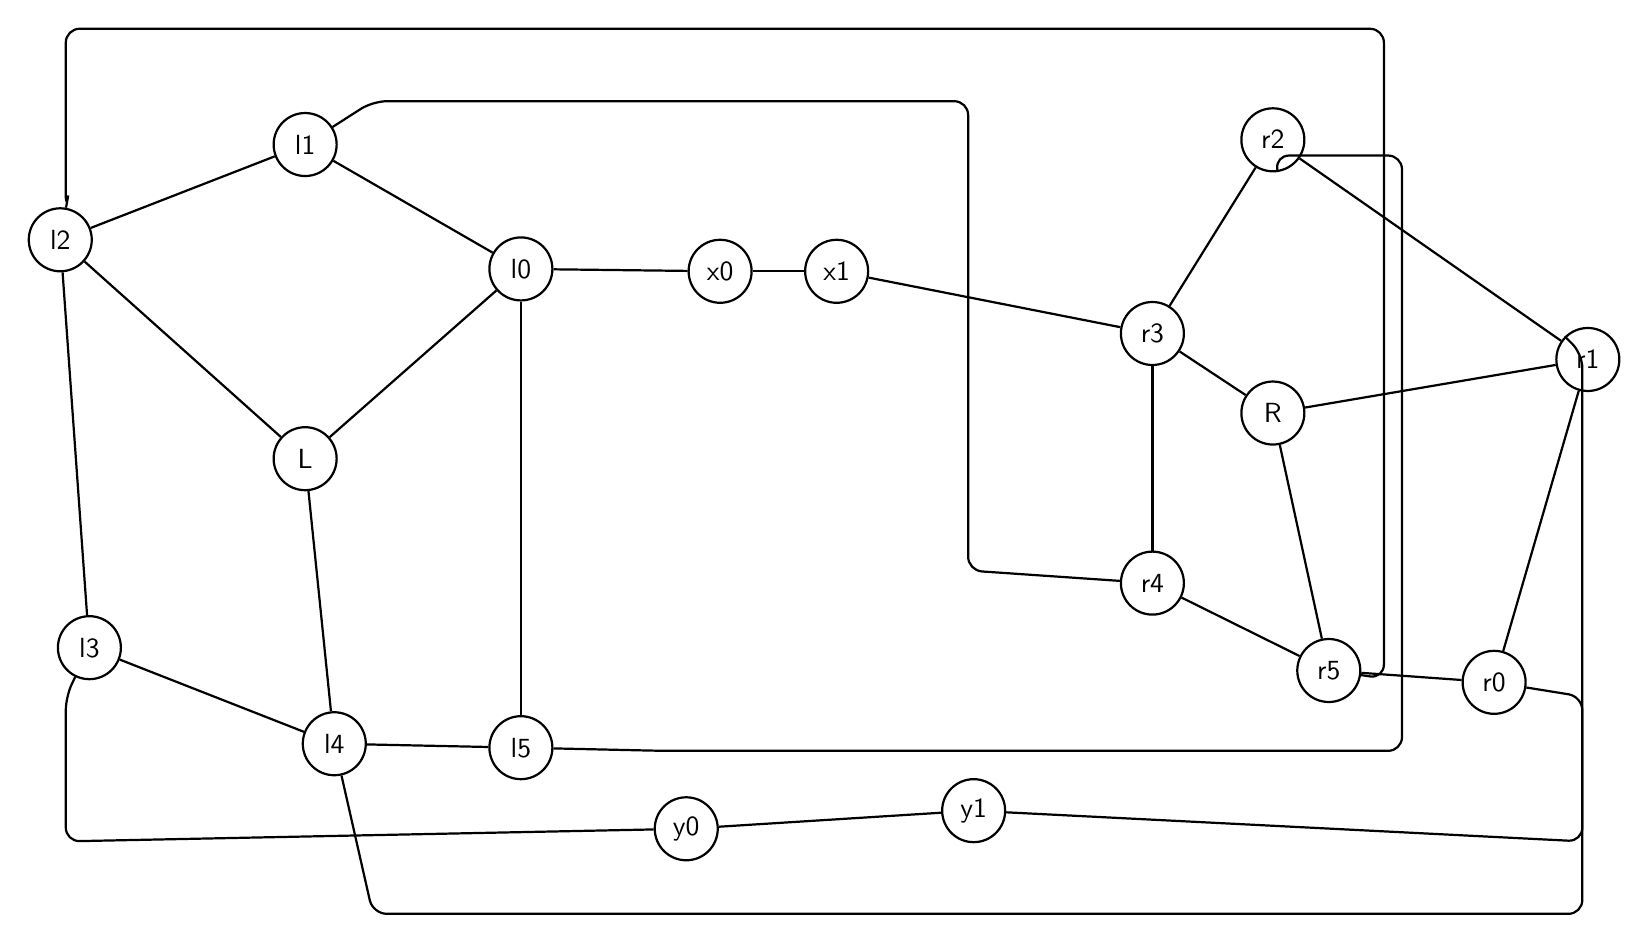
\begin{tikzpicture}[x=1cm,y=1cm]
\tikzset{
  graphnode/.style={circle,draw,thick,minimum size=8mm,inner sep=1pt,font=\sffamily},
  directed/.style={-{Stealth[length=2.4mm]},thick},
  undirected/.style={thick}
}
\node[graphnode] (n_L) at (-6.57,0.07) {L};
\node[graphnode] (n_l0) at (-3.83,2.48) {l0};
\node[graphnode] (n_l1) at (-6.57,4.06) {l1};
\node[graphnode] (n_l2) at (-9.68,2.85) {l2};
\node[graphnode] (n_l3) at (-9.31,-2.33) {l3};
\node[graphnode] (n_l4) at (-6.20,-3.55) {l4};
\node[graphnode] (n_l5) at (-3.83,-3.60) {l5};
\node[graphnode] (n_R) at (5.72,0.65) {R};
\node[graphnode] (n_r0) at (8.53,-2.77) {r0};
\node[graphnode] (n_r1) at (9.72,1.33) {r1};
\node[graphnode] (n_r2) at (5.72,4.12) {r2};
\node[graphnode] (n_r3) at (4.19,1.66) {r3};
\node[graphnode] (n_r4) at (4.19,-1.51) {r4};
\node[graphnode] (n_r5) at (6.43,-2.62) {r5};
\node[graphnode] (n_x0) at (-1.30,2.45) {x0};
\node[graphnode] (n_x1) at (0.18,2.45) {x1};
\node[graphnode] (n_y0) at (-1.73,-4.63) {y0};
\node[graphnode] (n_y1) at (1.92,-4.40) {y1};
\draw[undirected] (n_l0) -- (n_l1);
\draw[undirected] (n_l1) -- (n_l2);
\draw[undirected] (n_l2) -- (n_l3);
\draw[undirected] (n_l3) -- (n_l4);
\draw[undirected] (n_l4) -- (n_l5);
\draw[undirected] (n_l5) -- (n_l0);
\draw[undirected] (n_L) -- (n_l0);
\draw[undirected] (n_L) -- (n_l2);
\draw[undirected] (n_L) -- (n_l4);
\draw[undirected] (n_r0) -- (n_r1);
\draw[undirected] (n_r1) -- (n_r2);
\draw[undirected] (n_r2) -- (n_r3);
\draw[undirected] (n_r3) -- (n_r4);
\draw[undirected] (n_r4) -- (n_r5);
\draw[undirected] (n_r5) -- (n_r0);
\draw[undirected] (n_R) -- (n_r1);
\draw[undirected] (n_R) -- (n_r3);
\draw[undirected] (n_R) -- (n_r5);
\draw[undirected] (n_l0) -- (n_x0);
\draw[undirected] (n_x0) -- (n_x1);
\draw[undirected] (n_x1) -- (n_r3);
\draw[undirected,rounded corners=5pt] (n_l3) -- (-9.61,-2.95) -- (-9.61,-4.79) -- (n_y0);
\draw[undirected] (n_y0) -- (n_y1);
\draw[undirected,rounded corners=5pt] (n_y1) -- (9.65,-4.79) -- (9.65,-2.95) -- (n_r0);
\draw[undirected,rounded corners=5pt] (n_l1) -- (-5.71,4.61) -- (1.85,4.61) -- (1.85,-1.35) -- (n_r4);
\draw[undirected,rounded corners=5pt] (n_l2) -- (-9.61,3.24) -- (-9.61,5.53) -- (7.13,5.53) -- (7.13,-2.72) -- (n_r5);
\draw[undirected,rounded corners=5pt] (n_l4) -- (-5.71,-5.71) -- (9.65,-5.71) -- (9.65,1.40) -- (n_r1);
\draw[undirected,rounded corners=5pt] (n_l5) -- (-2.04,-3.64) -- (7.36,-3.64) -- (7.36,3.92) -- (5.75,3.92) -- (n_r2);
\end{tikzpicture}
\end{document}
